\PassOptionsToPackage{unicode=true}{hyperref} % options for packages loaded elsewhere
\PassOptionsToPackage{hyphens}{url}
%
\documentclass[]{article}
\usepackage{lmodern}
\usepackage{amssymb,amsmath}
\usepackage{ifxetex,ifluatex}
\usepackage{fixltx2e} % provides \textsubscript
\ifnum 0\ifxetex 1\fi\ifluatex 1\fi=0 % if pdftex
  \usepackage[T1]{fontenc}
  \usepackage[utf8]{inputenc}
  \usepackage{textcomp} % provides euro and other symbols
\else % if luatex or xelatex
  \usepackage{unicode-math}
  \defaultfontfeatures{Ligatures=TeX,Scale=MatchLowercase}
\fi
% use upquote if available, for straight quotes in verbatim environments
\IfFileExists{upquote.sty}{\usepackage{upquote}}{}
% use microtype if available
\IfFileExists{microtype.sty}{%
\usepackage[]{microtype}
\UseMicrotypeSet[protrusion]{basicmath} % disable protrusion for tt fonts
}{}
\IfFileExists{parskip.sty}{%
\usepackage{parskip}
}{% else
\setlength{\parindent}{0pt}
\setlength{\parskip}{6pt plus 2pt minus 1pt}
}
\usepackage{hyperref}
\hypersetup{
            pdftitle={AAaaa},
            pdfauthor={Sarah Meilinger},
            pdfborder={0 0 0},
            breaklinks=true}
\urlstyle{same}  % don't use monospace font for urls
\usepackage[margin=1in]{geometry}
\usepackage{graphicx,grffile}
\makeatletter
\def\maxwidth{\ifdim\Gin@nat@width>\linewidth\linewidth\else\Gin@nat@width\fi}
\def\maxheight{\ifdim\Gin@nat@height>\textheight\textheight\else\Gin@nat@height\fi}
\makeatother
% Scale images if necessary, so that they will not overflow the page
% margins by default, and it is still possible to overwrite the defaults
% using explicit options in \includegraphics[width, height, ...]{}
\setkeys{Gin}{width=\maxwidth,height=\maxheight,keepaspectratio}
\setlength{\emergencystretch}{3em}  % prevent overfull lines
\providecommand{\tightlist}{%
  \setlength{\itemsep}{0pt}\setlength{\parskip}{0pt}}
\setcounter{secnumdepth}{0}
% Redefines (sub)paragraphs to behave more like sections
\ifx\paragraph\undefined\else
\let\oldparagraph\paragraph
\renewcommand{\paragraph}[1]{\oldparagraph{#1}\mbox{}}
\fi
\ifx\subparagraph\undefined\else
\let\oldsubparagraph\subparagraph
\renewcommand{\subparagraph}[1]{\oldsubparagraph{#1}\mbox{}}
\fi

% set default figure placement to htbp
\makeatletter
\def\fps@figure{htbp}
\makeatother


\title{AAaaa}
\author{Sarah Meilinger}
\date{10/18/2020}

\begin{document}
\maketitle

Hello! I looked at PM from a station in Oakland, CA. Here are my
results.

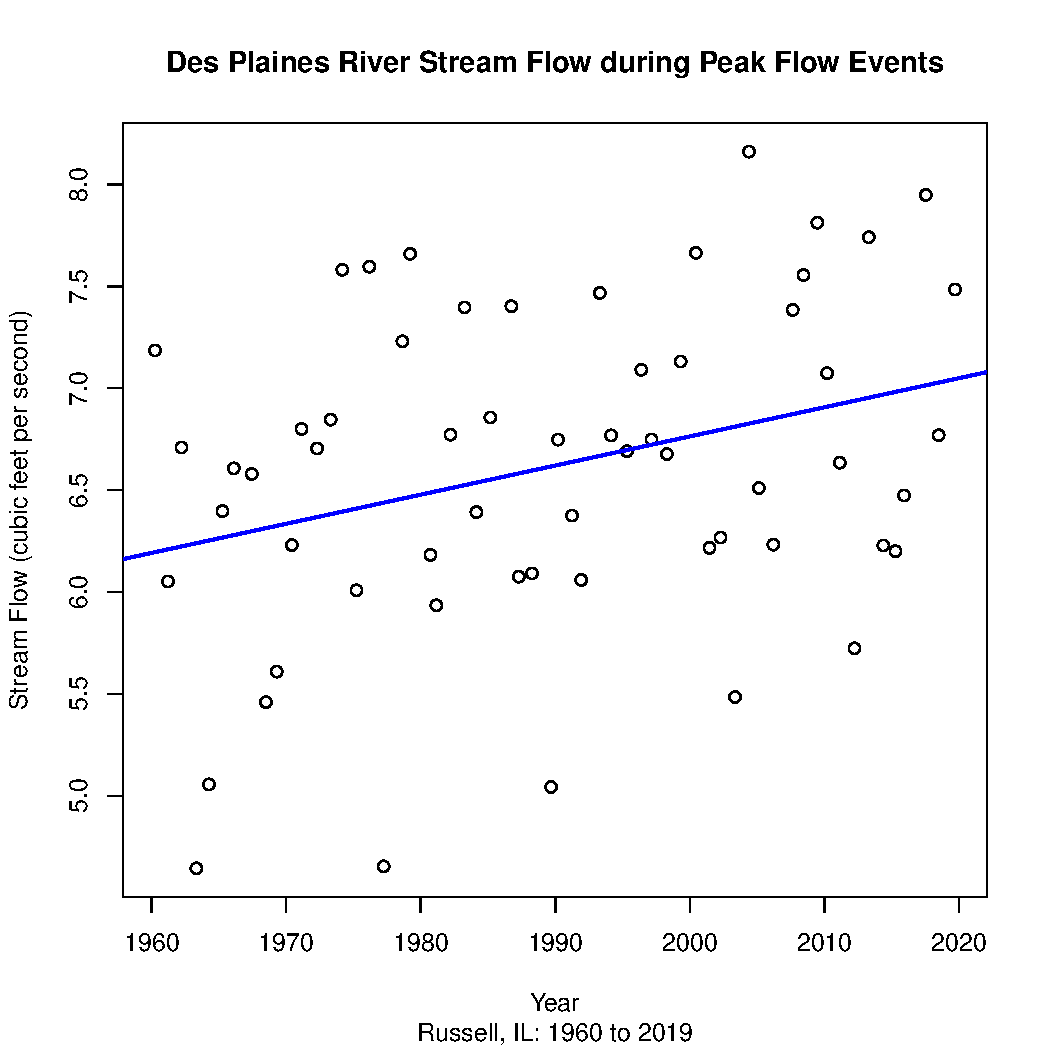
\includegraphics{Oakland-Last-Five-Years_files/figure-latex/unnamed-chunk-1-1.pdf}

\hypertarget{a-table-of-some-things-about-the-numbers}{%
\subsection{A table of some things about the
numbers}\label{a-table-of-some-things-about-the-numbers}}

This is a very crude table of Month \& mean \& standard deviation \& N
\& UCL95 \& LCL95

1.00 \& 10.20 \& 6.39 \& 155 \& 11.21 \& 9.20

2.00 \& 8.25 \& 4.95 \& 142 \& 9.07 \& 7.44

3.00 \& 6.88 \& 3.38 \& 153 \& 7.41 \& 6.34

4.00 \& 7.95 \& 3.94 \& 150 \& 8.58 \& 7.32

5.00 \& 7.89 \& 4.00 \& 155 \& 8.52 \& 7.26

6.00 \& 8.86 \& 4.14 \& 150 \& 9.52 \& 8.20

7.00 \& 8.70 \& 3.65 \& 154 \& 9.28 \& 8.13

8.00 \& 11.52 \& 7.47 \& 155 \& 12.70 \& 10.35

9.00 \& 16.26 \& 21.51 \& 145 \& 19.76 \& 12.76

10.00 \& 11.29 \& 9.35 \& 131 \& 12.89 \& 9.69

11.00 \& 18.78 \& 28.03 \& 120 \& 23.80 \& 13.77

12.00 \& 10.60 \& 7.88 \& 124 \& 11.99 \& 9.22

Some things of not are how both September and Novembers standard
deviations are relatively higher than the other months, and how most
charts have upper confidence limits of less than 15, excepting the month
of September, and all lower confidence limits are below 15, and most
below 10, excepting August, September, and November, at 10.35, 12.76,
and 13.77 respectively.

\hypertarget{health-good-no-health-bad}{%
\subsection{Health Good? No, Health
Bad}\label{health-good-no-health-bad}}

This graph shows the air frequently has particle matter of smaller than
2.5 µm over the recommended rate of 12 µg/m3. As Wu et al says in
\emph{Exposure to air pollution and COVID-19 mortality in the United
States: A nationwide cross-sectional study}, having ``an increase of 1
𝜇g/m3in long-term PM 2.5 exposure is associated with an 8\% increase in
the COVID-19 mortality rate'' (Wu et al). Thus, any amount of additional
PM2.5 above the recommended amount can have very negative effects on
health.

\hypertarget{thank-you}{%
\subsection{Thank You}\label{thank-you}}

Sarah Meilinger

\end{document}
